% HOW TO USE: do NOT replace the official NeurIPS template's main file. Open the official template
% (Formatting_Instructions_For_NeurIPS_2026.zip, upload it to Overleaf as a project), keep its preamble
% and its checklist at the end, and replace the example body with the lines below.

% --- extra packages (add to the template preamble if missing) ---
% \usepackage{booktabs}
% \usepackage{graphicx}
% \usepackage{amsmath}
% \usepackage{xcolor}
% \newcommand{\TODO}[1]{{\color{red}[TODO: #1]}}   % delete every \TODO before submitting

% --- title ---
% \title{A Small-Scale Check of Parameter-Counting Sensitivity in Chinchilla Compute-Optimal Scaling}

% --- body ---
% \begin{abstract}
%   \section{Results}
\label{sec:results}

% INSTRUCTIONS: run `python fit.py --boot 200`, then upload the contents of results/ to Overleaf
% (keep the folder name `results`). Write ONLY what the numbers show. Every \TODO below needs
% either a sentence supported by results/summary.json or deletion. Do not keep a sentence you
% cannot back with a number or a figure.

\subsection{IsoFLOP profiles}
Figure~\ref{fig:isoflop} shows validation loss against model size at each budget. \TODO{State whether each budget has an interior minimum, and at which model size. If the minimum sits at the smallest or largest size for some budget, say so: that budget is excluded from the Approach~2 fit.}

\begin{figure}[t]
  \centering
  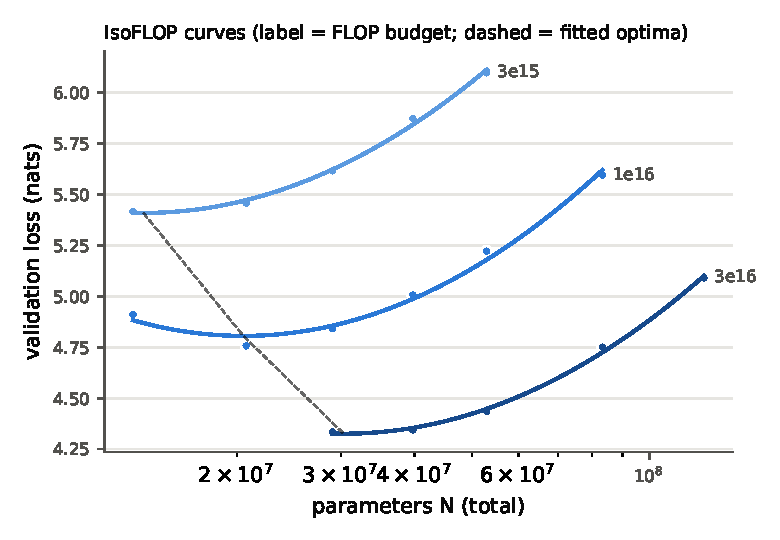
\includegraphics[width=0.75\linewidth]{results/fig_isoflop.pdf}
  \caption{IsoFLOP profiles: validation loss versus parameter count (total-parameter convention) at each FLOP budget. Curves are fitted parabolas in $\log N$; the dashed line connects the fitted minima.}
  \label{fig:isoflop}
\end{figure}

\subsection{Sensitivity to the parameter-counting convention (RQ1)}
Table~\ref{tab:conventions} and Figure~\ref{fig:exponents} report the fitted exponent $a$, the optimal token count $D^*(C_\text{ref})$ and $N^*(C_\text{ref})$ for each approach and convention. \TODO{Report: (i) how much $D^*$ changes across conventions for Approaches 2 and 3 (use \texttt{spreads} in summary.json), (ii) how much the exponent $a$ changes, (iii) whether the bootstrap intervals overlap. Remember Approach~1's $D^*$ is identical across conventions by construction. Then say whether the qualitative conclusion matches Schaeffer et al.}

\begin{table}[t]
  \centering
  \caption{Compute-optimal allocation at $C_\text{ref}$ under each approach and parameter-count convention. $a$ is the exponent in $N^*\propto C^a$. \TODO{Add bootstrap intervals if space allows.}}
  \label{tab:conventions}
  \begin{tabular}{llrrrr}
\toprule
Fit & $N$ convention & exponent $a$ & $D^*$ (M tok) & $N^*$ (M) & $D^*/N^*$ \\
\midrule
Envelope & total & 0.251 & 119 & 24.1 & 4.9 \\
Envelope & non-embedding & 0.674 & 119 & 2.0 & 61.2 \\
Envelope & excl.\ input emb. & 0.276 & 119 & 13.1 & 9.1 \\
IsoFLOP & total & 0.339 & 143 & 20.5 & 7.0 \\
IsoFLOP & non-embedding & 0.985 & 132 & 1.5 & 85.7 \\
IsoFLOP & excl.\ input emb. & 0.419 & 145 & 10.8 & 13.5 \\
Parametric & total & 0.139 & 163 & 18.3 & 8.9 \\
Parametric & non-embedding & 0.380 & 181 & 0.8 & 221.2 \\
Parametric & excl.\ input emb. & 0.160 & 159 & 9.8 & 16.2 \\
\bottomrule
\end{tabular}

\end{table}

\begin{figure}[t]
  \centering
  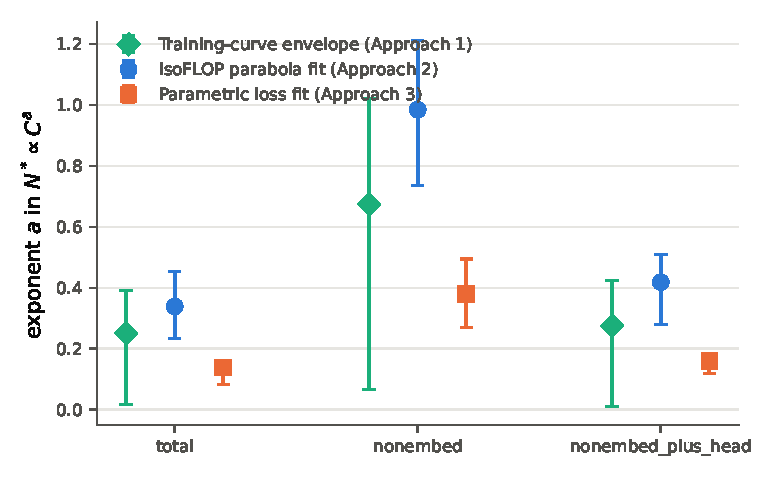
\includegraphics[width=0.75\linewidth]{results/fig_exponents.pdf}
  \caption{Fitted exponent $a$ by convention and approach, with bootstrap 95\% intervals. Intervals reflect which runs are included in the fit, not training-seed variation.}
  \label{fig:exponents}
\end{figure}

\subsection{Structured perturbations of the parameter counts (RQ1)}
Figure~\ref{fig:perturb} shows the optimal tokens-per-parameter ratio and the exponent $a$ under the four perturbations of Section~\ref{sec:perturb}. By construction a multiplicative constant leaves $D^*$ unchanged and rescales $N^*$ and the ratio exactly, so it serves as a check. \TODO{Report, from results/perturbation\_sweep.csv: how the exponent $a$ changes with the additive offset and with the bias slope for each approach (numbers), whether the ratio's trend with compute changes (column ratio\_slope), how large the effect of log-normal noise is relative to the draw-to-draw spread, and whether this agrees in direction with what Schaeffer et al.\ report. Do not claim agreement or disagreement beyond what the numbers show.}

\begin{figure}[t]
  \centering
  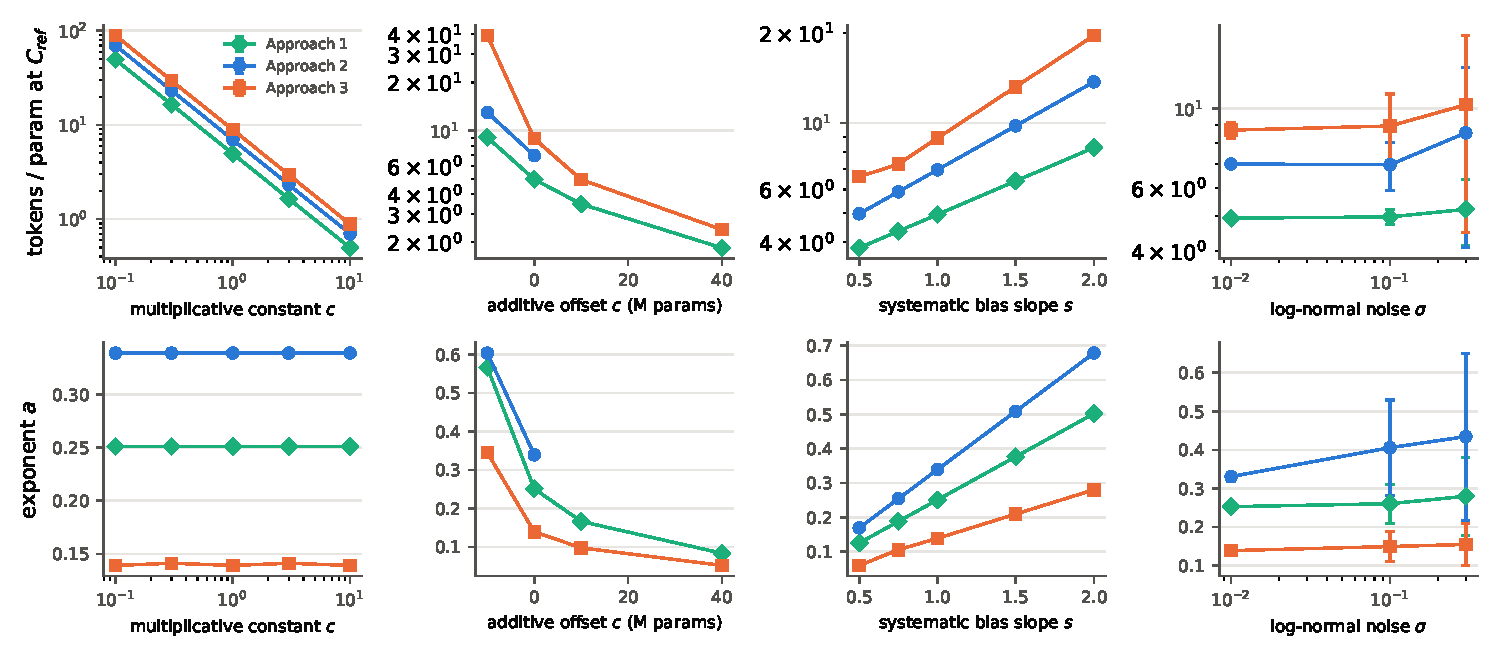
\includegraphics[width=\linewidth]{results/fig_perturbation.pdf}
  \caption{Effect of structured perturbations of the parameter counts (columns: multiplicative, additive, systematic bias, log-normal noise) on the optimal tokens-per-parameter ratio at the reference budget (top) and on the exponent $a$ (bottom), for each approach. Error bars for the noise column are standard deviations over 10 draws.}
  \label{fig:perturb}
\end{figure}

\subsection{Comparison of the three approaches (RQ3)}
\TODO{Use \texttt{approach\_gap} in summary.json: for each convention, the gap in $a$ and the relative gap in $D^*$ between each pair of approaches. State which pair agrees best and which worst, with numbers.}

\subsection{Shrinking the fitting grid (RQ2)}
Figure~\ref{fig:shrink} shows the spread of the exponent across conventions as the grid shrinks. \TODO{Using shrink\_sweep.csv, state whether the spread grows when budgets or sizes are removed, and at what point a fit fails entirely (no interior minimum, fewer than two valid budgets). If there is no clear trend with this few subsets, say so plainly.}

\begin{figure}[t]
  \centering
  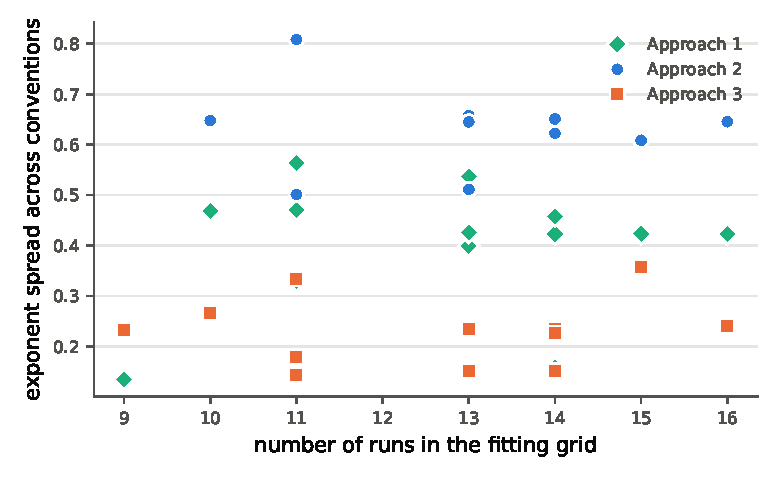
\includegraphics[width=0.75\linewidth]{results/fig_shrink.pdf}
  \caption{Spread of the exponent $a$ across parameter-count conventions for each subset of the grid, against the number of runs retained.}
  \label{fig:shrink}
\end{figure}

% \end{abstract}
% \section{Limitations}
\label{sec:limitations}

\begin{itemize}
  \item \textbf{Scale.} Our models have 0.39M--59M non-embedding parameters and our budgets span about one order of magnitude, orders of magnitude below the runs studied by Hoffmann et al.\ and others. Conclusions may not transfer to larger scales.
  \item \textbf{Embedding-dominated models.} With a 50k-token vocabulary, embedding and output-head parameters dominate the smallest models. This makes the parameter-counting conventions differ much more here than at larger scale, so differences across conventions should not be read as an estimate of the effect at scale.
  \item \textbf{Single seed and untuned hyperparameters.} Each configuration is trained once, and learning rates follow an untuned heuristic. Bootstrap intervals capture fitting variability across runs, not training noise or hyperparameter sensitivity.
  \item \textbf{Few data points.} Fits use \TODO{15} runs. The parametric fit has five free parameters, and the IsoFLOP fits use three to five points per budget, so intervals are wide.
  \item \textbf{Discrete model sizes.} Approach~1 selects among seven fixed sizes, which makes its estimates coarse.
  \item \textbf{Our own conventions and compute accounting.} The parameter-count conventions and the FLOPs formula are our definitions and may differ from those of the papers we compare against. We evaluate optima at a reference budget inside the grid, but exponents are extrapolated beyond it when used for larger budgets.
  \item \textbf{Not a re-analysis of Chinchilla's data.} We do not re-fit Hoffmann et al.'s published data or reproduce Schaeffer et al.'s three interpretations of the reported model sizes; our parameter-count conventions differ from theirs, and we apply their structured perturbations to our own fitted allocations. As in their analysis, perturbations change only $N$, not $D$ or the losses.
  \item \textbf{One dataset and tokenizer.} All experiments use C4 and the GPT-2 tokenizer.
\end{itemize}

% \section{Conclusion}
\label{sec:conclusion}

% Write 4--6 sentences AFTER the results are in. Restate only findings that the numbers support,
% answer RQ1--RQ3 in one sentence each, and point to the limitations (Section~\ref{sec:limitations}).
\TODO{Summarise what the small-scale replication shows about the sensitivity of compute-optimal allocation to the parameter-counting convention, how the three approaches compare, and how stable the conclusions are as the grid shrinks.}

% \begin{tabular}{lrrrrrrr}
\toprule
Size & Layers & $d_\text{model}$ & Heads & Non-emb.\ (M) & Non-emb.+head (M) & Total (M) & MFLOPs/token \\
\midrule
t0 & 2 & 128 & 2 & 0.39 & 6.8 & 13.3 & 42 \\
t1 & 3 & 192 & 3 & 1.33 & 11.0 & 20.7 & 68 \\
s0 & 4 & 256 & 4 & 3.15 & 16.0 & 29.0 & 99 \\
s1 & 6 & 320 & 5 & 7.38 & 23.5 & 39.7 & 147 \\
s2 & 8 & 384 & 6 & 14.17 & 33.5 & 53.0 & 210 \\
s3 & 10 & 512 & 8 & 31.48 & 57.2 & 83.3 & 359 \\
s4 & 12 & 640 & 10 & 59.01 & 91.2 & 123.7 & 571 \\
\bottomrule
\end{tabular}

% \section{Introduction}
\label{sec:intro}

Training a large language model requires deciding, before the run starts, how to split a fixed compute budget $C$ between the number of model parameters $N$ and the number of training tokens $D$. Kaplan et al.~\citep{kaplan2020} first fit power laws for pre-training loss as a function of $N$ and $D$; Hoffmann et al.~\citep{hoffmann2022} revisited the question by training over 400 models and concluded that $N$ and $D$ should be scaled roughly in equal proportion, which became the widely cited rule of about 20 training tokens per parameter.

Several follow-up studies have questioned details of this result. Besiroglu et al.~\citep{besiroglu2024} attempted to replicate one of Hoffmann et al.'s three estimation approaches and reported inconsistencies in the published fit. Porian et al.~\citep{porian2024} and Pearce and Song~\citep{pearce2024} examined why the Kaplan and Hoffmann prescriptions differ, with the choice of how to count parameters (for example, whether embedding parameters are included) playing a role in the explanation. Most recently, Schaeffer et al.~\citep{schaeffer2025} refit the parametric loss on Chinchilla's data under three ways of computing the model sizes (the published counts, a formula assuming tied embeddings, and a best-fit variant of the formula; these counts differ by up to 15.2\%) and under four structured perturbations of the counts (multiplicative, additive, size-dependent bias, and log-normal noise). They report that the choice among the three interpretations does not meaningfully change the estimates or the roughly 20-to-1 token-to-parameter ratio, while additive or systematic errors can bias the fitted exponents and change the trend of the optimal ratio with compute.

These analyses rely on large training runs or on re-analysis of published data. It is less clear how such a robustness analysis behaves in the small-scale regime that a practitioner with limited compute can actually reproduce, where embedding and output-head parameters make up a large fraction of the model. We therefore ask:
\begin{itemize}
  \item \textbf{RQ1 (reproduction).} Do the sensitivities Schaeffer et al.\ report, in particular to additive offsets of the parameter count (counting or excluding embedding parameters acts like one) and to size-dependent bias, appear at small scale, where embedding parameters are a large share of the model?
  \item \textbf{RQ2 (boundary conditions).} As the fitting grid shrinks (fewer model sizes, fewer budgets), when do the conclusions stop being stable?
  \item \textbf{RQ3 (estimation approaches).} How do Hoffmann et al.'s three estimation approaches compare under each convention?
\end{itemize}

\paragraph{Contributions.} (i) A small-scale, fully open analogue of the parameter-counting analysis of Schaeffer et al., applying their four structured perturbations to our own fitted allocations with all three Hoffmann et al.\ estimation approaches. (ii) A grid-shrinking sweep that probes how the conclusions degrade with less data. (iii) Code and a recovery test on synthetic data with a known scaling law. \TODO{Edit contributions to match what the results actually support.}

% \section{Results}
\label{sec:results}

% INSTRUCTIONS: run `python fit.py --boot 200`, then upload the contents of results/ to Overleaf
% (keep the folder name `results`). Write ONLY what the numbers show. Every \TODO below needs
% either a sentence supported by results/summary.json or deletion. Do not keep a sentence you
% cannot back with a number or a figure.

\subsection{IsoFLOP profiles}
Figure~\ref{fig:isoflop} shows validation loss against model size at each budget. \TODO{State whether each budget has an interior minimum, and at which model size. If the minimum sits at the smallest or largest size for some budget, say so: that budget is excluded from the Approach~2 fit.}

\begin{figure}[t]
  \centering
  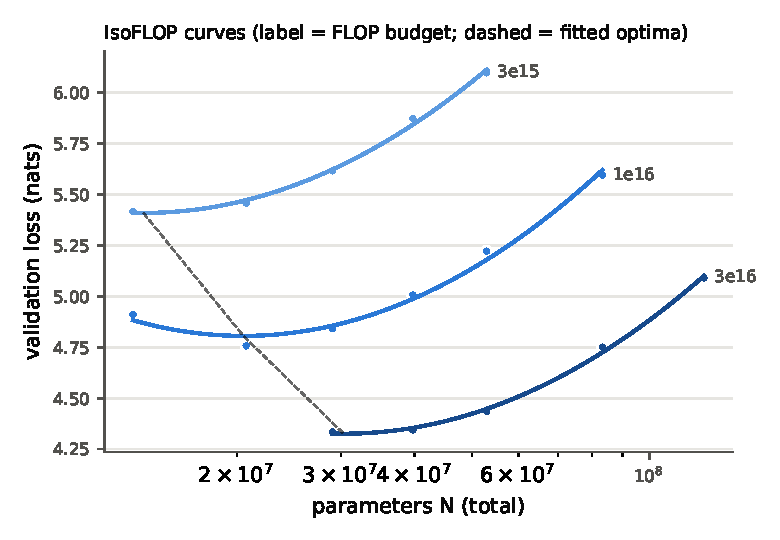
\includegraphics[width=0.75\linewidth]{results/fig_isoflop.pdf}
  \caption{IsoFLOP profiles: validation loss versus parameter count (total-parameter convention) at each FLOP budget. Curves are fitted parabolas in $\log N$; the dashed line connects the fitted minima.}
  \label{fig:isoflop}
\end{figure}

\subsection{Sensitivity to the parameter-counting convention (RQ1)}
Table~\ref{tab:conventions} and Figure~\ref{fig:exponents} report the fitted exponent $a$, the optimal token count $D^*(C_\text{ref})$ and $N^*(C_\text{ref})$ for each approach and convention. \TODO{Report: (i) how much $D^*$ changes across conventions for Approaches 2 and 3 (use \texttt{spreads} in summary.json), (ii) how much the exponent $a$ changes, (iii) whether the bootstrap intervals overlap. Remember Approach~1's $D^*$ is identical across conventions by construction. Then say whether the qualitative conclusion matches Schaeffer et al.}

\begin{table}[t]
  \centering
  \caption{Compute-optimal allocation at $C_\text{ref}$ under each approach and parameter-count convention. $a$ is the exponent in $N^*\propto C^a$. \TODO{Add bootstrap intervals if space allows.}}
  \label{tab:conventions}
  \begin{tabular}{llrrrr}
\toprule
Fit & $N$ convention & exponent $a$ & $D^*$ (M tok) & $N^*$ (M) & $D^*/N^*$ \\
\midrule
Envelope & total & 0.251 & 119 & 24.1 & 4.9 \\
Envelope & non-embedding & 0.674 & 119 & 2.0 & 61.2 \\
Envelope & excl.\ input emb. & 0.276 & 119 & 13.1 & 9.1 \\
IsoFLOP & total & 0.339 & 143 & 20.5 & 7.0 \\
IsoFLOP & non-embedding & 0.985 & 132 & 1.5 & 85.7 \\
IsoFLOP & excl.\ input emb. & 0.419 & 145 & 10.8 & 13.5 \\
Parametric & total & 0.139 & 163 & 18.3 & 8.9 \\
Parametric & non-embedding & 0.380 & 181 & 0.8 & 221.2 \\
Parametric & excl.\ input emb. & 0.160 & 159 & 9.8 & 16.2 \\
\bottomrule
\end{tabular}

\end{table}

\begin{figure}[t]
  \centering
  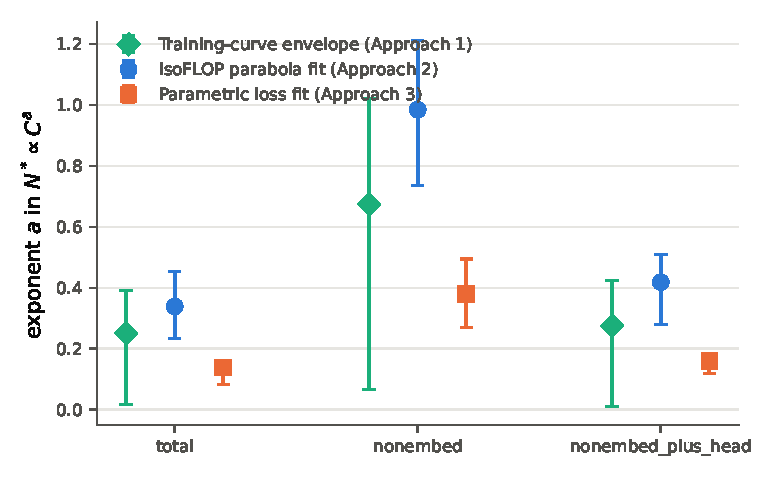
\includegraphics[width=0.75\linewidth]{results/fig_exponents.pdf}
  \caption{Fitted exponent $a$ by convention and approach, with bootstrap 95\% intervals. Intervals reflect which runs are included in the fit, not training-seed variation.}
  \label{fig:exponents}
\end{figure}

\subsection{Structured perturbations of the parameter counts (RQ1)}
Figure~\ref{fig:perturb} shows the optimal tokens-per-parameter ratio and the exponent $a$ under the four perturbations of Section~\ref{sec:perturb}. By construction a multiplicative constant leaves $D^*$ unchanged and rescales $N^*$ and the ratio exactly, so it serves as a check. \TODO{Report, from results/perturbation\_sweep.csv: how the exponent $a$ changes with the additive offset and with the bias slope for each approach (numbers), whether the ratio's trend with compute changes (column ratio\_slope), how large the effect of log-normal noise is relative to the draw-to-draw spread, and whether this agrees in direction with what Schaeffer et al.\ report. Do not claim agreement or disagreement beyond what the numbers show.}

\begin{figure}[t]
  \centering
  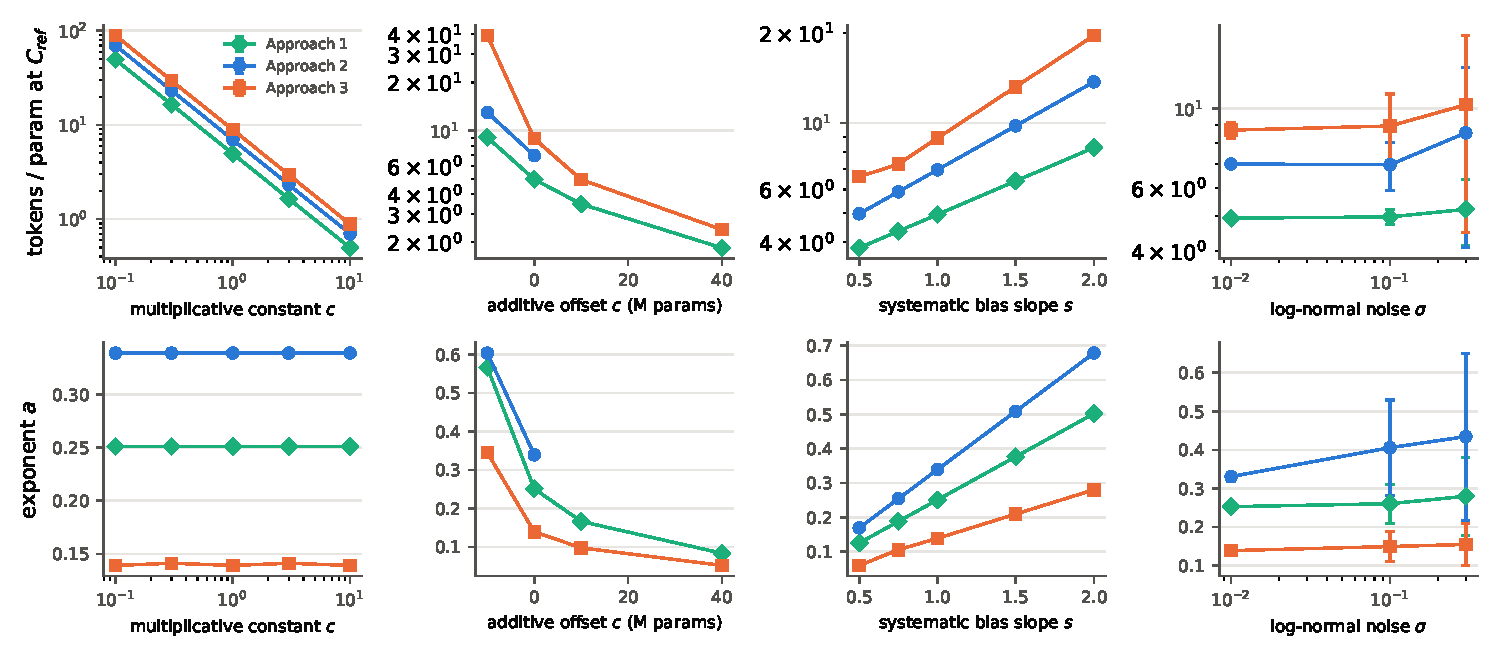
\includegraphics[width=\linewidth]{results/fig_perturbation.pdf}
  \caption{Effect of structured perturbations of the parameter counts (columns: multiplicative, additive, systematic bias, log-normal noise) on the optimal tokens-per-parameter ratio at the reference budget (top) and on the exponent $a$ (bottom), for each approach. Error bars for the noise column are standard deviations over 10 draws.}
  \label{fig:perturb}
\end{figure}

\subsection{Comparison of the three approaches (RQ3)}
\TODO{Use \texttt{approach\_gap} in summary.json: for each convention, the gap in $a$ and the relative gap in $D^*$ between each pair of approaches. State which pair agrees best and which worst, with numbers.}

\subsection{Shrinking the fitting grid (RQ2)}
Figure~\ref{fig:shrink} shows the spread of the exponent across conventions as the grid shrinks. \TODO{Using shrink\_sweep.csv, state whether the spread grows when budgets or sizes are removed, and at what point a fit fails entirely (no interior minimum, fewer than two valid budgets). If there is no clear trend with this few subsets, say so plainly.}

\begin{figure}[t]
  \centering
  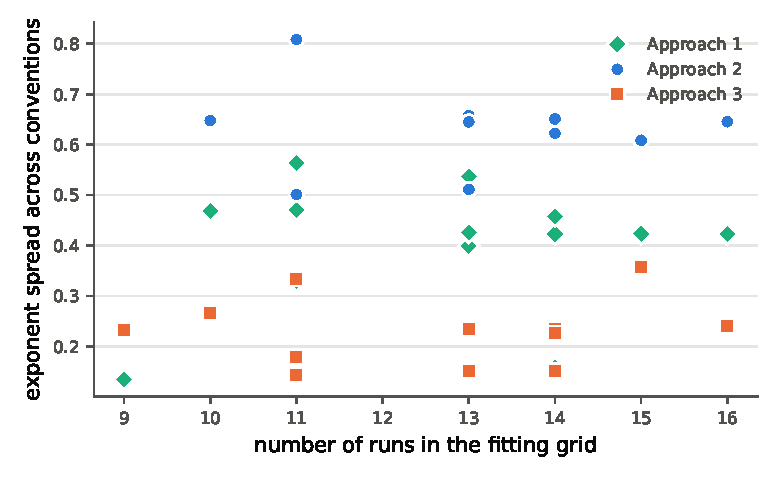
\includegraphics[width=0.75\linewidth]{results/fig_shrink.pdf}
  \caption{Spread of the exponent $a$ across parameter-count conventions for each subset of the grid, against the number of runs retained.}
  \label{fig:shrink}
\end{figure}

% \begin{tabular}{lrrrr}
\toprule
Budget $C$ (FLOPs) & Size & Tokens $D$ (M) & Steps & Tokens / non-emb.\ param \\
\midrule
3e15 & t0 & 71.8 & 2191 & 182.0 \\
3e15 & t1 & 44.3 & 1353 & 33.3 \\
3e15 & s0 & 30.2 & 922 & 9.6 \\
3e15 & s1 & 20.4 & 624 & 2.8 \\
3e15 & s2 & 14.3 & 435 & 1.0 \\
1e16 & t1 & 147.8 & 4509 & 111.1 \\
1e16 & s0 & 100.7 & 3074 & 32.0 \\
1e16 & s1 & 68.2 & 2080 & 9.2 \\
1e16 & s2 & 47.5 & 1451 & 3.4 \\
1e16 & s3 & 27.9 & 850 & 0.9 \\
3e16 & s0 & 302.2 & 9221 & 95.9 \\
3e16 & s1 & 204.5 & 6240 & 27.7 \\
3e16 & s2 & 142.7 & 4354 & 10.1 \\
3e16 & s3 & 83.6 & 2550 & 2.6 \\
3e16 & s4 & 52.6 & 1604 & 0.9 \\
\bottomrule
\end{tabular}

% \section{Method}
\label{sec:method}

\paragraph{Notation.} $N$ is a parameter count (defined by a convention below), $D$ the number of training tokens, $C$ the training compute in FLOPs, and $L$ the validation cross-entropy loss in nats per token. A starred quantity ($N^*$, $D^*$) is compute-optimal for a given $C$.

\subsection{Models and compute accounting}
We train decoder-only Transformers in the GPT-2 style~\citep{radford2019gpt2}: pre-LayerNorm blocks, GELU MLP with 4$\times$ expansion, learned positional embeddings, no biases in linear layers, untied input and output embeddings, context length 512, and a GPT-2 byte-pair-encoding vocabulary padded to 50{,}304 tokens. We use seven model sizes (Table~\ref{tab:sizes}) with head dimension 64.

Training FLOPs per token are computed analytically as
\begin{equation}
  f(N) = 6\left(12\,n_\text{layer}\,d_\text{model}^2 + d_\text{model} V\right) + 6\,n_\text{layer}\,T\,d_\text{model},
\end{equation}
where $V$ is the vocabulary size and $T$ the context length; the first term counts matrix multiplications in the blocks and the output head (forward plus backward), the second counts causal attention. Embedding lookups cost no FLOPs. The total compute of a run is $C = D\,f$. Note that $f$ is \emph{not} proportional to any single parameter count here, because the output head contributes FLOPs but not block parameters.

\subsection{Parameter-count conventions}
\label{sec:conventions}
We compare three conventions: (\textbf{total}) all parameters; (\textbf{non-embedding}) transformer blocks and final LayerNorm only; (\textbf{non-embedding + head}) everything except the input token and position embeddings. These conventions are ours. They differ from the three interpretations of Schaeffer et al.~\citep{schaeffer2025}, which are three ways of computing the sizes of Chinchilla's models (the published counts, a formula assuming tied embeddings and no positional embeddings, and a best-fit variant of the attention term) that differ by at most 15.2\%. We compare embedding-based conventions because embedding parameters are the dominant ambiguity at our scale, and because including or excluding them acts like an additive offset to $N$, one of the perturbations Schaeffer et al.\ study.

\subsection{Training}
Each run uses AdamW~\citep{loshchilov2019adamw} with $\beta=(0.9, 0.95)$, weight decay 0.1 on matrices, gradient clipping at 1.0, bfloat16 autocast, and 32{,}768 tokens per optimizer step (gradient accumulation over micro-batches of 16 sequences). The learning rate follows linear warm-up (between 10 and 200 steps) and cosine decay to 10\% of the peak, scheduled over each run's own length, which is the setting IsoFLOP-style fits assume. The peak learning rate is set by the untuned heuristic $\min(2\times10^{-3},\,6\times10^{-4}\cdot 768/d_\text{model})$. Training data are consumed once in order, so no token is repeated. Each configuration is trained with a single random seed.

\subsection{Estimating compute-optimal allocations}
\label{sec:fits}
For each convention we apply the three approaches of Hoffmann et al.\ to the same runs. Every approach yields a power law $N^* \propto C^{a}$ and $D^* \propto C^{b}$; we additionally report $N^*$ and $D^*$ at a reference budget $C_\text{ref}$, the geometric mean of the budgets in the grid.

\paragraph{Approach 1: training-curve envelope.} Each run's validation loss is recorded about eight times during training. We interpolate each run's curve linearly in $\log C$ and, at every $C$ on a dense grid where at least two model sizes are available, select the run with the lowest loss. We regress $\log N$ and $\log D$ of the selected runs on $\log C$. Because intermediate points come from runs whose learning rate has not finished decaying, and because the choice is among discrete model sizes, this approach is coarse.

\paragraph{Approach 2: IsoFLOP profiles.} For every budget with at least three runs, we fit a parabola to loss as a function of $\log N$ and take its minimum as $N^*$ (requiring an interior minimum); $D^*$ is interpolated from the runs at the same budget. We then regress $\log N^*$ and $\log D^*$ on $\log C$.

\paragraph{Approach 3: parametric loss surface.} We fit $L(N,D) = E + A N^{-\alpha} + B D^{-\beta}$ to all runs by minimizing the Huber loss ($\delta = 10^{-3}$) of the log-residuals with L-BFGS-B from 162 initializations. For a budget $C$, the optimum minimizes $L(N, C/f(N))$ over $N$, where $f(N)$ is a log-log linear fit of FLOPs per token against $N$ across the model ladder. This makes the optimum consistent with the actual compute accounting for every convention.

\subsection{Robustness metrics and uncertainty}
\label{sec:robust}
For each approach we report, across conventions, the spread of the exponent $a$ (maximum minus minimum) and the relative spread of $D^*(C_\text{ref})$, which is a physical quantity (a token count) and therefore comparable across conventions, whereas $N^*$ and $a$ depend on how $N$ is defined. Pairwise gaps between approaches address RQ3. Approach~1 selects runs by loss alone, so its $D^*$ does not depend on the convention by construction.

We quantify fitting uncertainty with a bootstrap (\TODO{200} resamples): runs are resampled with replacement within each budget (Approaches 1 and 2) or overall (Approach 3), and we report percentile 95\% intervals. These intervals capture variation due to which runs are included, \emph{not} variation due to training seeds.

\subsection{Structured perturbations of the parameter counts}
\label{sec:perturb}
Following Schaeffer et al.~\citep{schaeffer2025}, we perturb the parameter counts of the total-parameter convention in four ways and refit all three approaches each time, leaving $D$ and the losses untouched: (i) a multiplicative constant, $N\to cN$, $c\in\{0.1,0.3,1,3,10\}$; (ii) an additive constant, $N\to N+c$, $c\in\{-10,0,10,40\}$M; (iii) a systematic bias that stretches $\log N$ around its geometric mean with slope $s\in\{0.5,0.75,1,1.5,2\}$; and (iv) log-normal noise, $N\to e^{\delta}N$ with $\delta\sim\mathcal N(0,\sigma^2)$, $\sigma\in\{0.01,0.1,0.3\}$, averaged over 10 draws. Because a counting error is a property of the architecture, each perturbation is applied per model size, so all runs of one size share it. Where Schaeffer et al.\ assume $C\approx cND$ with an unspecified constant, we keep the exact FLOPs accounting $f(N)$, recomputed from the perturbed counts. We report the optimal tokens-per-parameter ratio and the exponent $a$ at each level.

\paragraph{Grid-shrinking sweep (RQ2).} We repeat the analysis after removing each budget in turn, each model size in turn, the two extreme sizes, and every other size, and track the spread across conventions as a function of the number of runs.

\paragraph{Validation on a known law.} To check the fitting code, we generate synthetic runs from a known law and verify that all three approaches recover its optimal allocation (see Appendix).

%
% \bibliographystyle{plainnat}   % use the style the template recommends if it differs
% \bibliography{references}
%
% \newpage
% % ABSTRACT -- fill every \TODO after running fit.py. Keep to ~150-200 words.
Hoffmann et al.\ (2022) fixed the field's default recipe for allocating a training compute budget between model size and training tokens (``Chinchilla'', roughly 20 tokens per parameter). Schaeffer et al.\ (2025) recently stress-tested this recipe: they found that the conclusion is insensitive to how Chinchilla's model sizes are computed, but can be affected by additive or size-dependent errors in the parameter counts. We carry out a small-scale analogue of this analysis on a single consumer GPU. We train \TODO{15} GPT-style language models (0.39M--59M non-embedding parameters) on C4 at \TODO{three} FLOP budgets ($3\times10^{15}$--$3\times10^{16}$) and fit all three of Hoffmann et al.'s estimation approaches (training-curve envelope, IsoFLOP parabolas, parametric loss surface) under three parameter-count conventions (total, non-embedding, non-embedding plus output head), and apply four structured perturbations to the parameter counts following Schaeffer et al. \TODO{One sentence: the main finding about how the fitted optimal token count $D^*$ and exponent $a$ change across conventions.} \TODO{One sentence: how the three approaches compare.} A grid-shrinking sweep shows that \TODO{one sentence: when the conclusions become unstable as the fitting grid shrinks.} Code is released to support replication.

%
% % The NeurIPS Paper Checklist from the template goes AFTER the appendix and must stay (papers without
% % it are desk-rejected). Fill it using checklist_answers.md.

% Files to upload to Overleaf: sections/, tables/, references.bib, and the contents of results/
% (after running fit.py) as a folder named `results`.
